%! TeX program = lualatex
%---------------------------ALLGEMEINE IMPORTS-------------------------------------
\documentclass[12pt,english,ngerman]{scrartcl}
\input{./protokoll_template/template.latex/input/shared_preamble.tex}

% Kopfzeile
\ihead{WS22\\
	21.12.2022} \chead{\textsc{Stark} Matthias - 12004907 \\
	\textsc{Philipp} Maximilian - 11839611}
\ohead{FLAB 1 \\
	Rasterelektronenmikroskopie}
% Fußzeile


\begin{document}

\section{Grundlagen}

%(max. 1 Seite)


\section{Proben- und Geräteliste}


\section{Kennenlernen des REM}


Zunächst wird die Probe mit einer Pinzette vorsichtig auf den Probentisch platziert. Für ein effektives Arbeiten können 
mehrere Proben gleichzeitig auf die Probenbühne gesetzt und diese zwischen den einzelnen Messungen einfach weitergedreht
werden. Im Rahmen des Praktikums wird jedoch immer nur eine Probe eingelegt, um das Handling zu lernen und sicherzustellen,
dass die "z-Ebene", also die Höhe, immer richtig eingestellt ist. Die Orientierung in dei "z-Achse" wird fixiert, um 
sicherzustellen, dass kein "crash" verursacht wird.

Bei der Probe ist zu beachten, dass diese elektrisch leitfähig sein muss. Ist die Probe von sich aus schon leitfähig, wird
sie mit einem speziellen, leitenden Kohlenstoff-Band am Sockel befestigt. Handelt es sich um eine nicht leitende Probe, so 
muss die leitfähigkeit z.B. durch eine Platin Bedampfung gewährleistet werden, wie im \autoref{fig:probe} sichtbar.

\begin{figure}[H]
	\begin{center}
		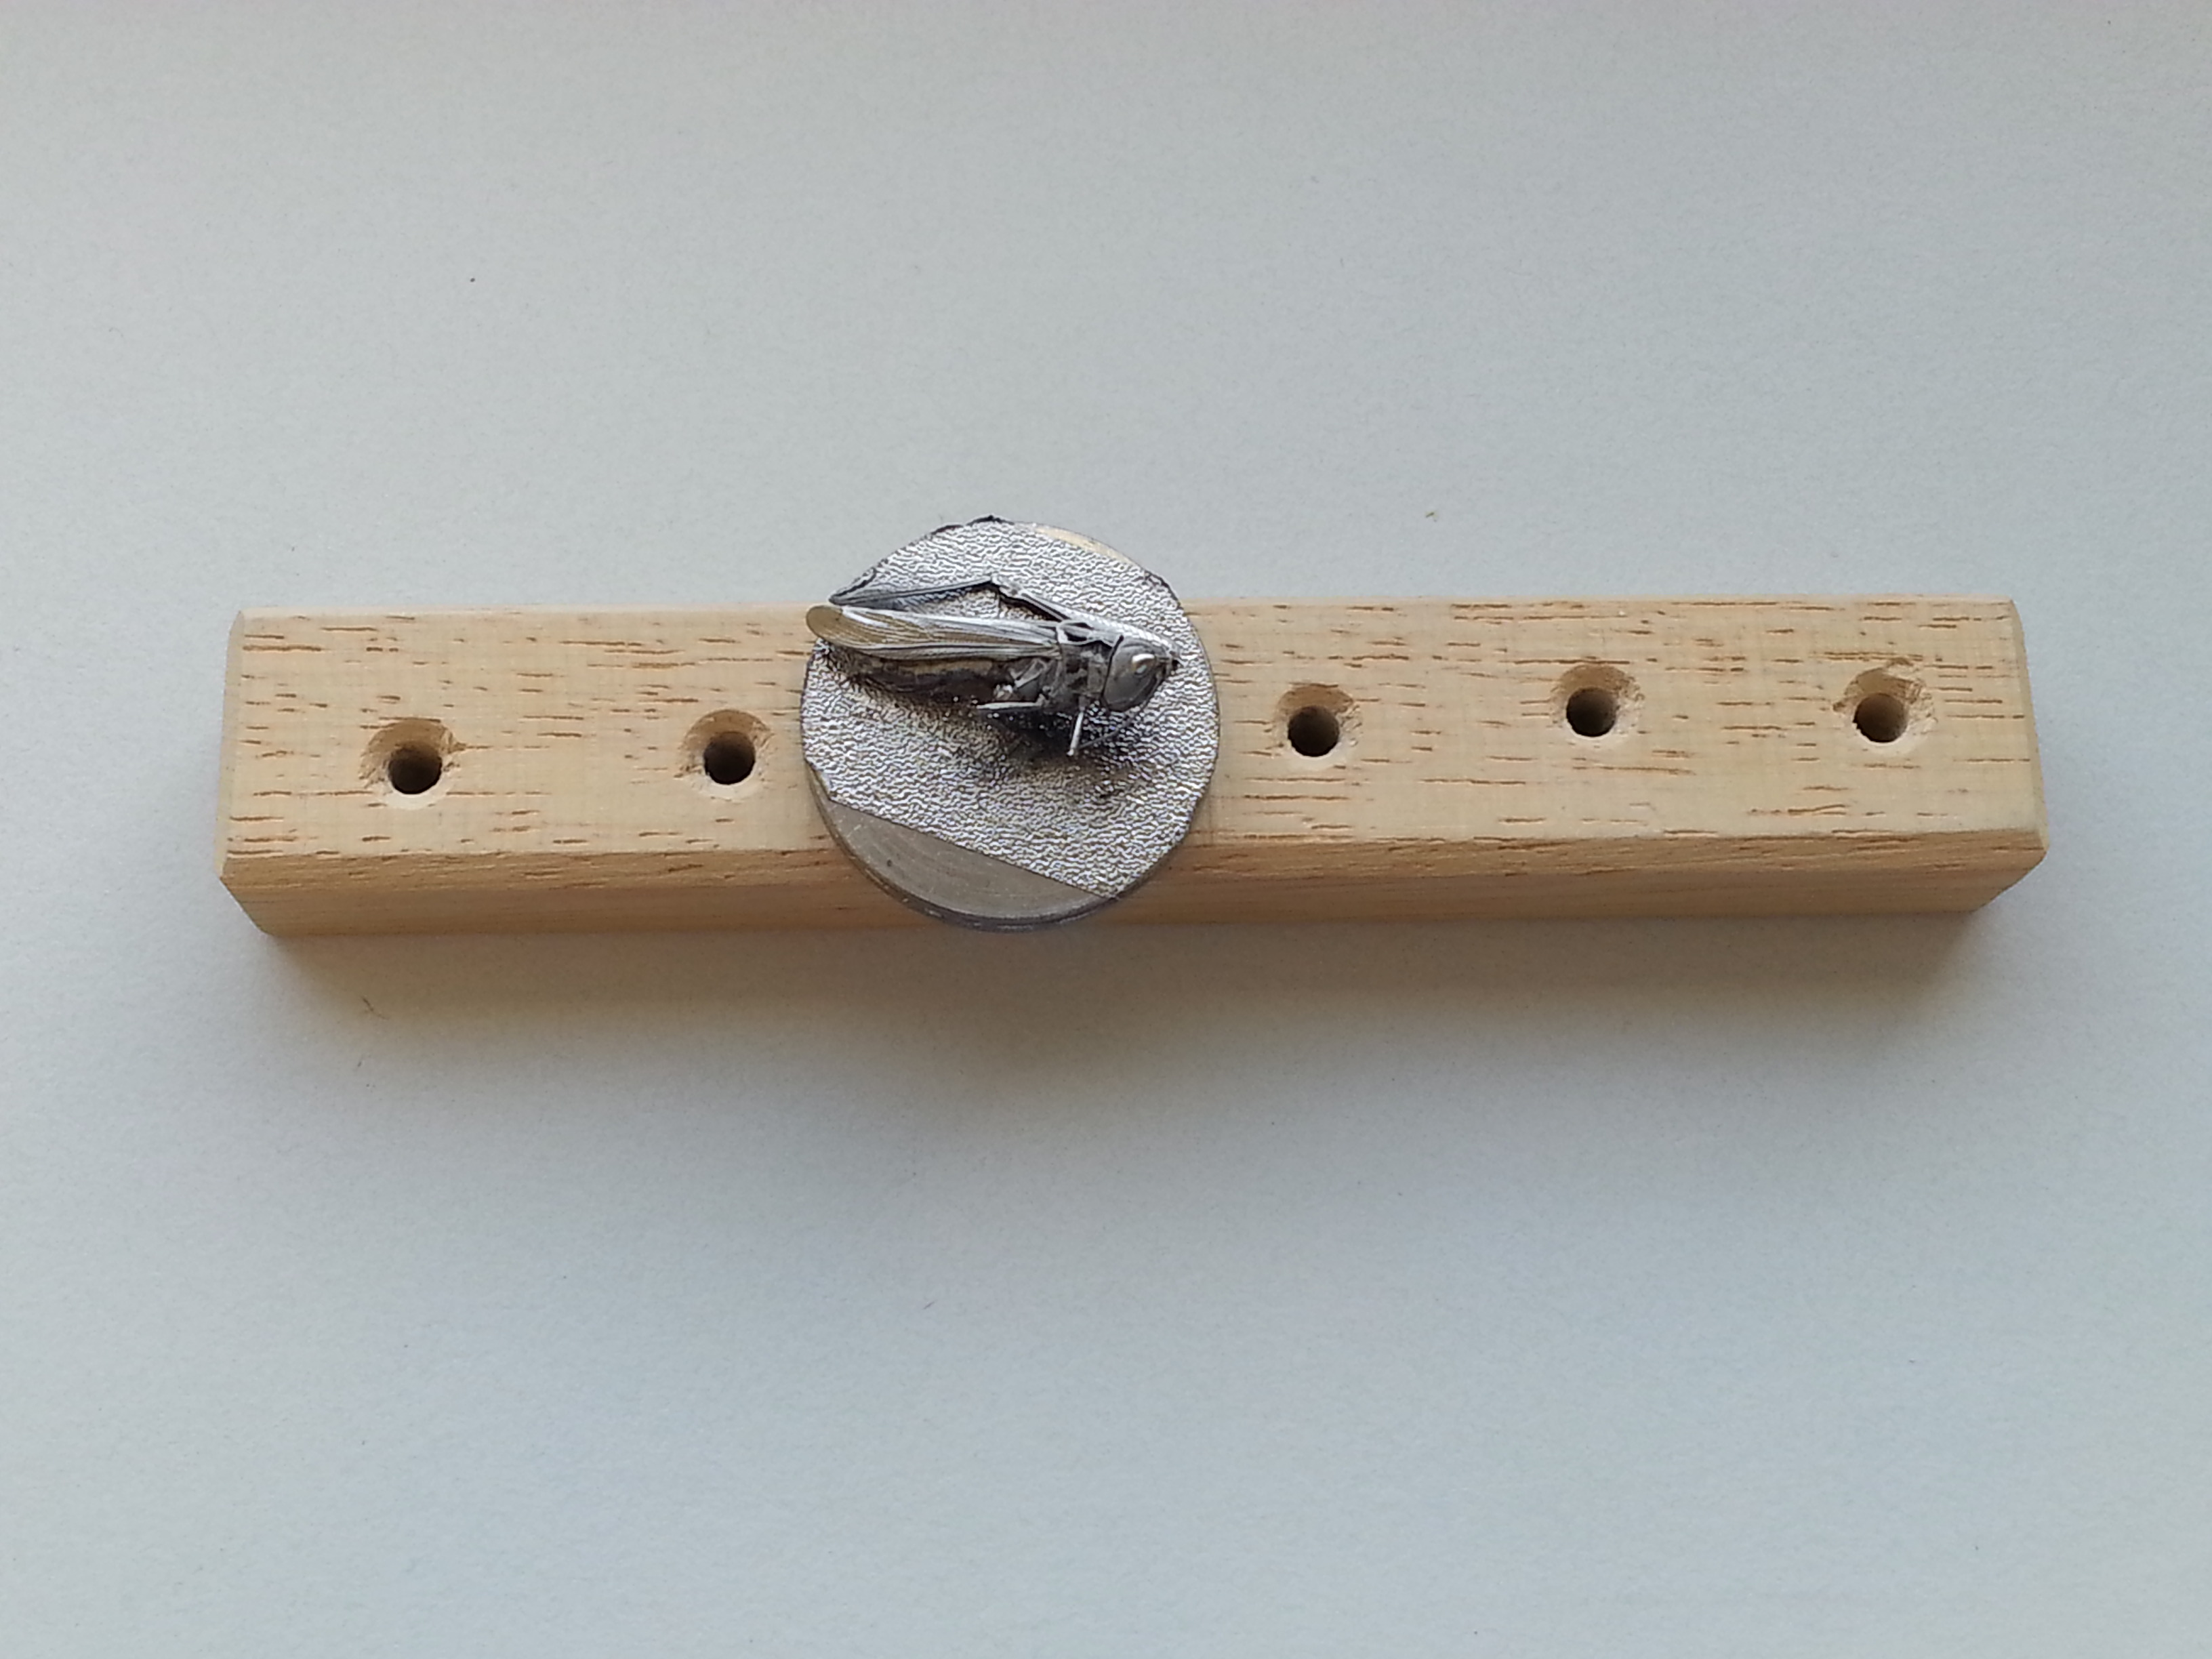
\includegraphics[width =0.5\textwidth]{./figures/probe.png}
	\end{center}
	\caption[Bedampfte, organische Probe]
	{Bedampfte, organische Probe \cite{sein_foto}}
    \label{fig:probe}
\end{figure}

Nach dem Einlegen der Probe wird ein Vakuum erzeugt, welches für den Betrieb des Elektronenmikroskops notwendig ist, was 
\SI{162(1)}{\s}, also keine \SI{3}{\min} dauert.

Nun wird das aufgezeichnete Bild im verwendeten Computerprogramm sichtbar. Durch Bewegung mit der Computermaus kann 
der entsprechende Bereich ausgewählt und die Vergrößerung eingestellt werden. Auch kann über den entsprechenden Knopf die 
Schärfe, sowie der Kontrast, variiert werden, um ein möglichst gut aufgelöstes Bild zu erreichen. Man muss sich bewusst 
sein, dass wie bei allen
optischen Aufbauten, gewisse Abbildungsfehler vorliegen. Für eine genauere Erklärung hierzu, sein auf \cite{unterlagen} 
verwiesen. Der Astigmatismus durch eine entsprechende Anpassung im jeweiligen Menüpunkt großteils behoben werden.


%todo gets vlt dass wir jeweils 2 Bilder nebeneinander kriegen? 

Im folgenden ist eine Auswahl der erzeugten Bilder angeführt. In \autoref{fig:auge} und \autoref{fig:auge2} sind Aufnahmen
des Facettenauges sichtbar. In \autoref{fig:flugel} sieht man die Struktur des Flügels und in \autoref{fig:damage} ist eine
komisch geformte Struktur sichtbar, die auf einen Fehler in der Bedampfungsschicht zurückzuführen ist.

\begin{figure}[H]
	\begin{center}
		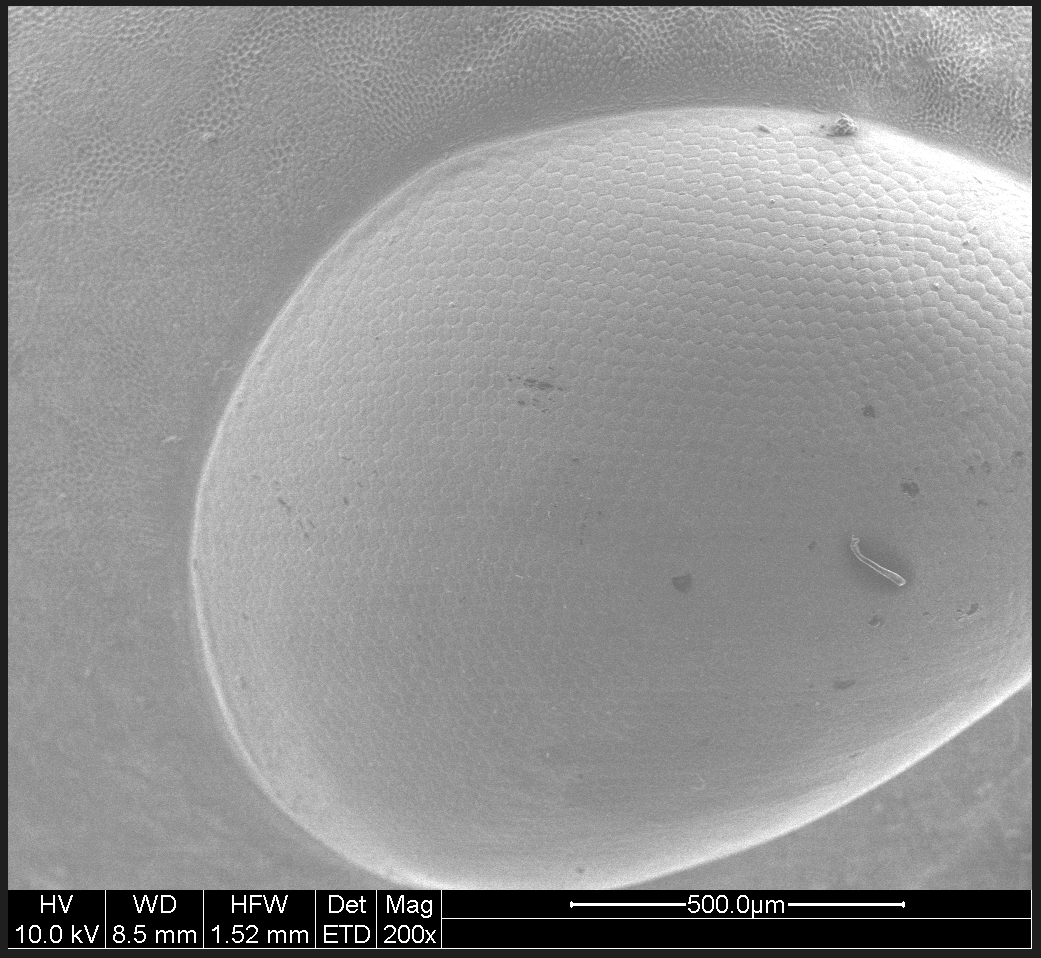
\includegraphics[width =0.5\textwidth]{./figures/auge.png}
	\end{center}
	\caption{Facettenauge}
    \label{fig:auge}
\end{figure}

\begin{figure}[H]
	\begin{center}
		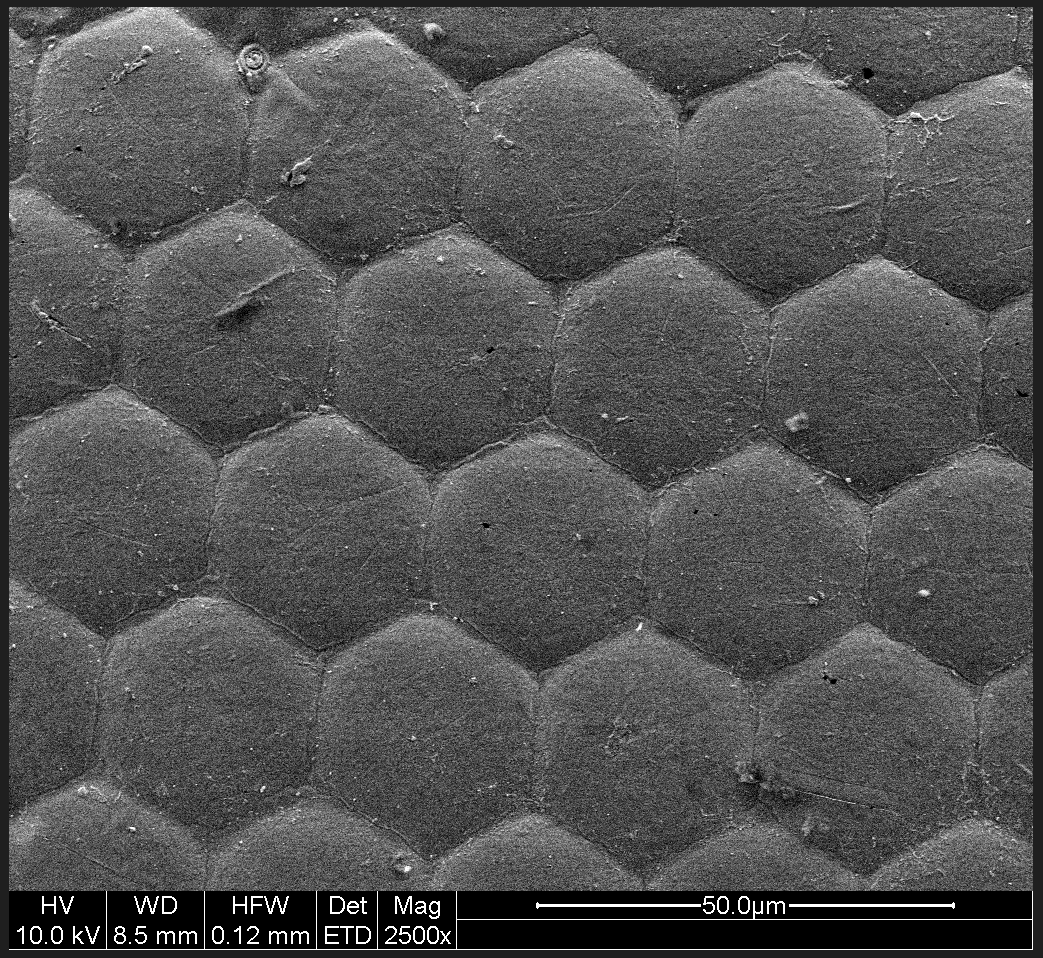
\includegraphics[width =0.5\textwidth]{./figures/auge2.png}
	\end{center}
	\caption{stärker vergrößertes Facettenauge}
    \label{fig:auge2}
\end{figure}

\begin{figure}[H]
	\begin{center}
		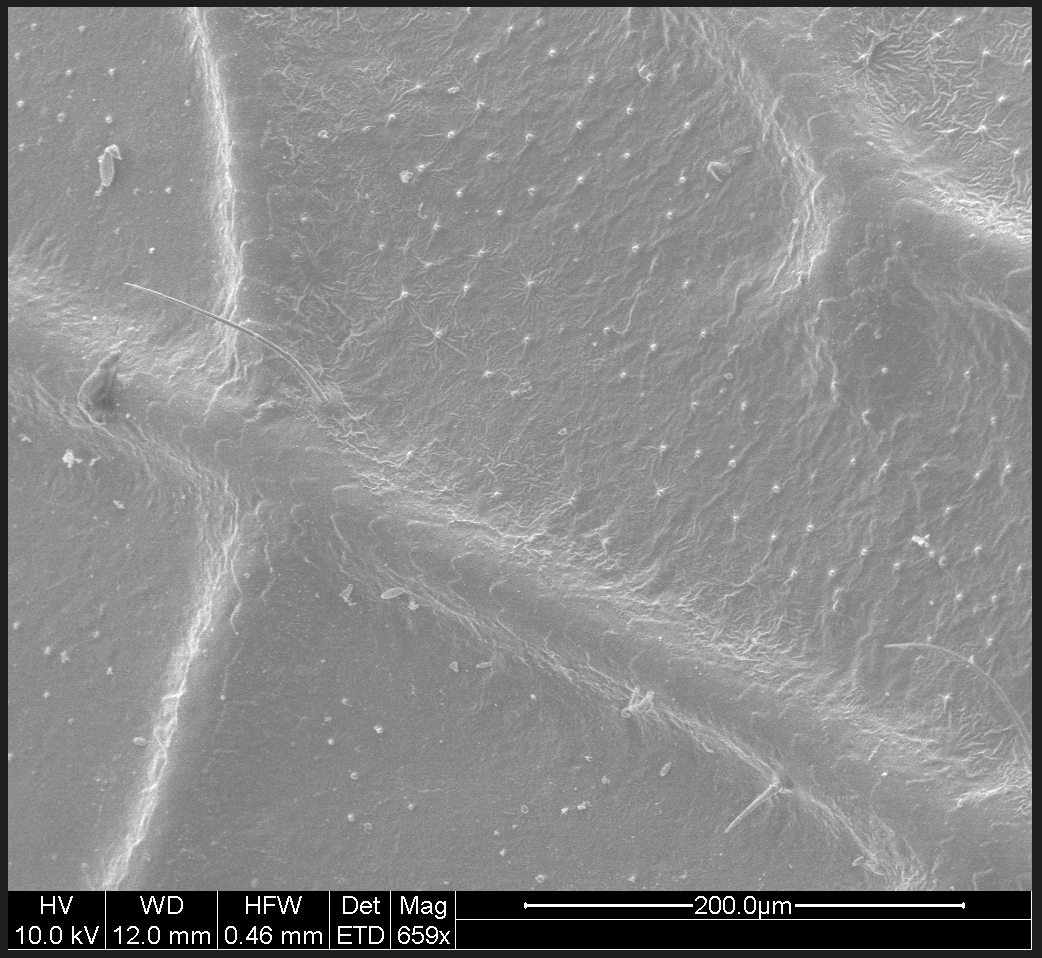
\includegraphics[width =0.5\textwidth]{./figures/flugel.png}
	\end{center}
	\caption{Struktur des Flügels}
    \label{fig:flugel}
\end{figure}

\begin{figure}[H]
	\begin{center}
		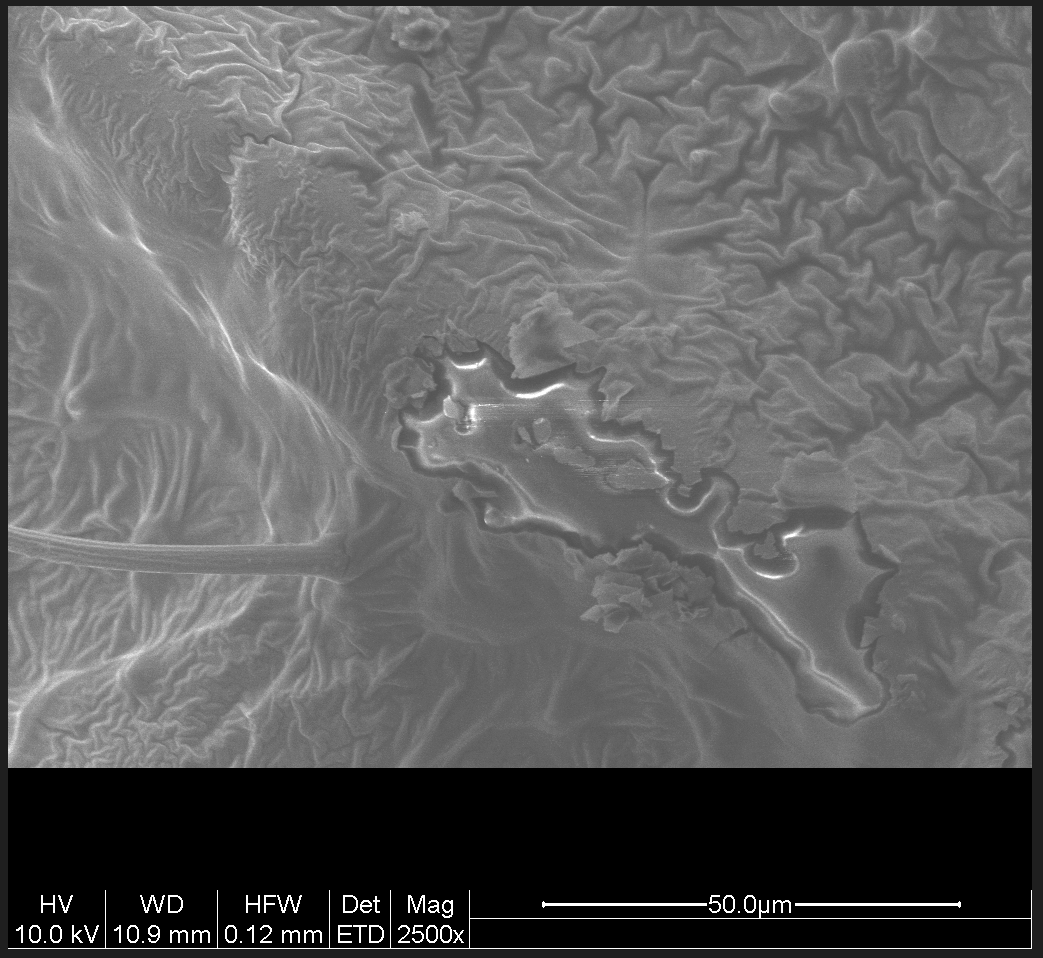
\includegraphics[width =0.5\textwidth]{./figures/damage.png}
	\end{center}
	\caption{Fehler in Bedampfungsschicht}
    \label{fig:damage}
\end{figure}


\section{Polypropylen-Gewebe}

Nun wird ein teilweise beschichtetes Stück eines Polypropylen Gewebes in den Aufbau gegeben, wie in \autoref{fig:aufbau} sichtbar.

\begin{figure}[H]
	\begin{center}
		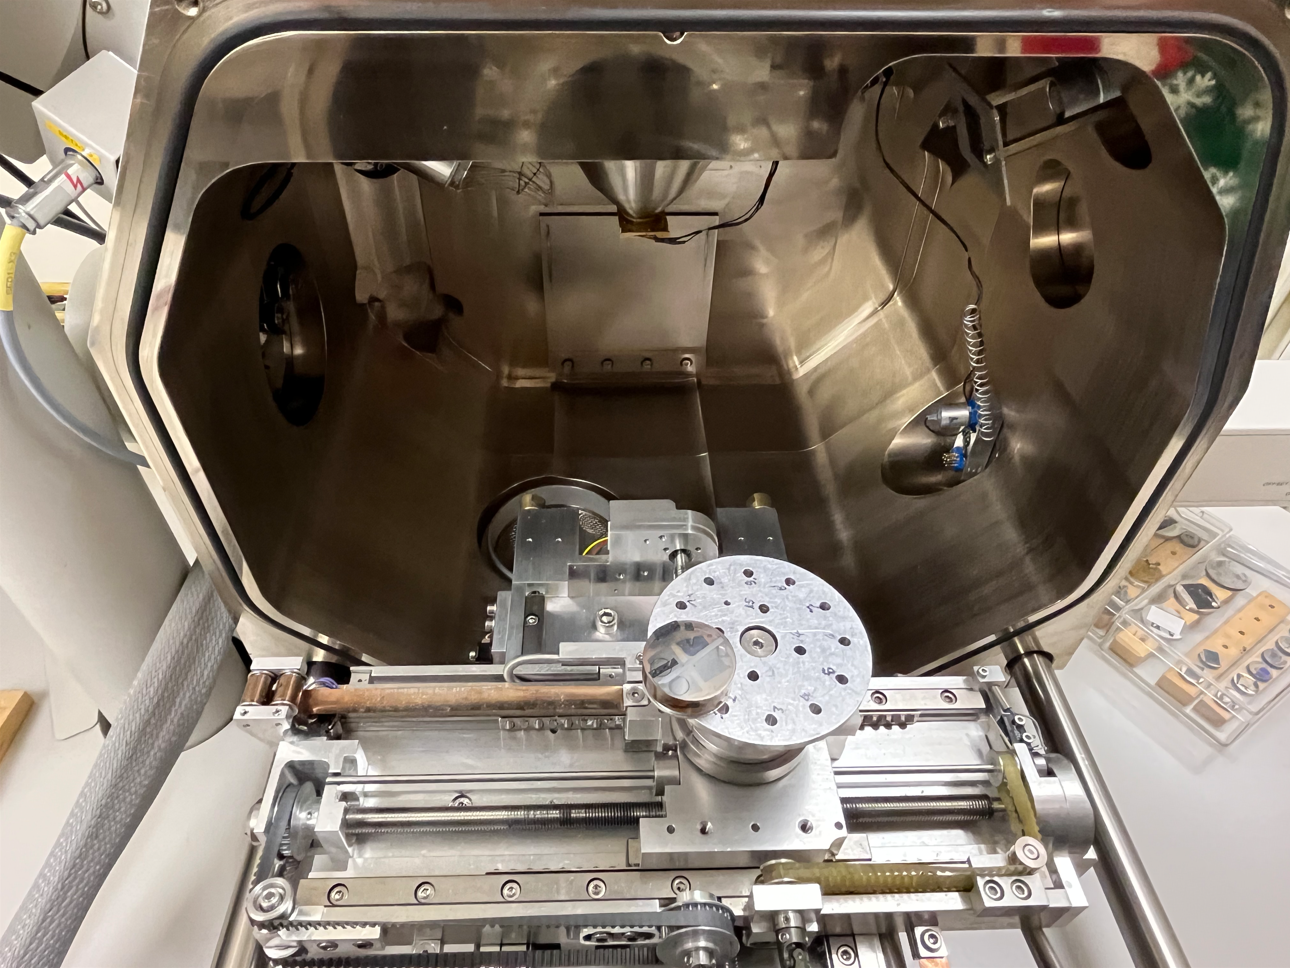
\includegraphics[width =0.5\textwidth]{./figures/aufbau.png}
	\end{center}
	\caption{Polypropylen Gewebe in Versuchsaufbau}
    \label{fig:aufbau}
\end{figure}


\subsection{Vergleich „beschichtet“ und „unbeschichtet“}

Zunächst dir jeweils eine Beschichtete und eine un beschichtete Position auf der Probe als Position markiert, um einen
unproblematischen Wechsel zwischen ihnen zu ermöglichen. Die Betrachtung der erzeugten Bilder zeigt sofort, dass im 
beschichteten Zustand viel schärfere Fotos erzeugt werden können, wie im nächsten Kapitel ersichtlich. Betrachtet man 
den unbeschichteten Zustand, wie in \autoref{fig:unbeschichtet} sichtbar, wird deutlich, dass am Präparat feine 
Bewegungen der Struktur sichtbar sind, was an den ruckartigen Unterbrechungen in folgender \autoref{fig:unbeschichtet}
sichtbar wird. Besonders leicht erkennbar werden diese Bewegungen, wenn mehrere Bilder aufgezeichnet werden und diese 
dann als Film abgespielt werden, was im Rahmen dieses Protokolls aber leider nicht geteilt werden kann.
\begin{figure}[H]
	\begin{center}
		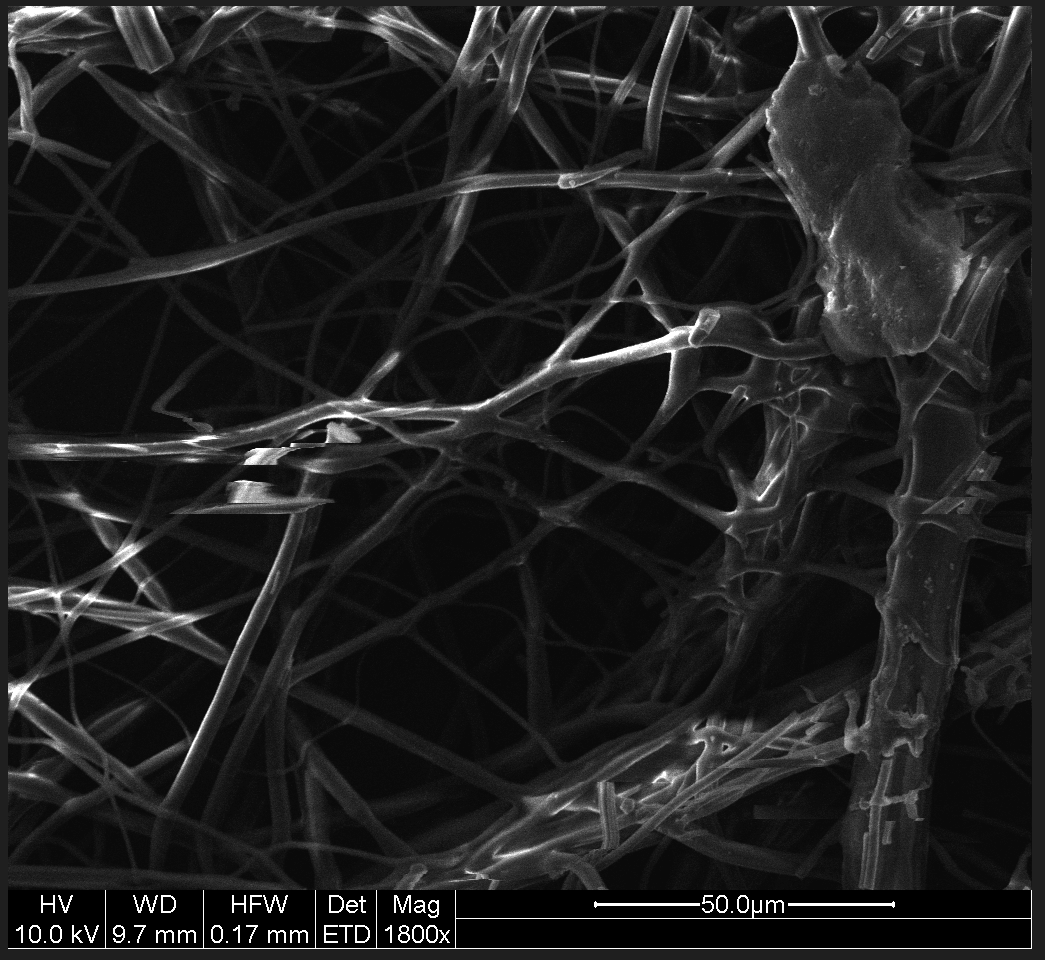
\includegraphics[width =0.5\textwidth]{./figures/unbedampft.png}
	\end{center}
	\caption{Unbeschichtetes Polypropylen Gewebe}
    \label{fig:unbeschichtet}
\end{figure}

\subsection{Variation der Beschleunigungsspannung}


\section{Keramik}


\subsection{Vergleich SE- und BSE-Abbildung}


\subsection{Bestimmung der Schichtdicke}


\section{Qualitative EDX-Analyse}


\section{Quantitative EDX-Analyse}


\section{Zusammenfassung}


\section{Anhang}


%Vorbereitungsunterlagen, Daten über Münzen



\newpage

\printbibliography

\end{document}